\documentclass{article}

\usepackage{amsmath, amsthm, amssymb, amsfonts}
\usepackage{thmtools}

% ------------------------------------------------------------------------------
\usepackage{graphicx}
\graphicspath{ {./images/} }
% ------------------------------------------------------------------------------

\usepackage{setspace}
\usepackage{geometry}
\usepackage{float}
\usepackage{hyperref}
\usepackage[english]{babel}
\usepackage{framed}
\usepackage[dvipsnames]{xcolor}
\usepackage{tcolorbox}
\usepackage{minted}

% ------------------------------------------------------------------------------
% \usepackage{times}
% \usepackage{fontspec}
% \setmainfont{Ubuntu Nerd Font}
% \setsansfont{Noto Sans}
% \setmonofont{FiraCode Nerd Font}
% ------------------------------------------------------------------------------

\colorlet{LightGray}{White!90!Periwinkle}
\colorlet{LightOrange}{Orange!15}
\colorlet{LightGreen}{Green!15}

\newcommand{\HRule}[1]{\rule{\linewidth}{#1}}

\declaretheoremstyle[name=Theorem,]{thmsty}
\declaretheorem[style=thmsty,numberwithin=section]{theorem}
\tcolorboxenvironment{theorem}{colback=LightGray}

\declaretheoremstyle[name=Proposition,]{prosty}
\declaretheorem[style=prosty,numberlike=theorem]{proposition}
\tcolorboxenvironment{proposition}{colback=LightOrange}

\declaretheoremstyle[name=Principle,]{prcpsty}
\declaretheorem[style=prcpsty,numberlike=theorem]{principle}
\tcolorboxenvironment{principle}{colback=LightGreen}

\setstretch{1.2}
\geometry{
    textheight=9in,
    textwidth=5.5in,
    top=1in,
    headheight=12pt,
    headsep=25pt,
    footskip=30pt
}

% ------------------------------------------------------------------------------

\begin{document}

% ------------------------------------------------------------------------------
% Cover Page and ToC
% ------------------------------------------------------------------------------

\title{ \normalsize \textsc{}
\\ [2.0cm]
\HRule{1.5pt} \\
\LARGE \textbf{\uppercase{Data Communications and
	Networking}
\HRule{2.0pt} \\ [0.6cm] \LARGE{Chapter 08} \vspace*{10\baselineskip}}
}
\date{}
\author{\textbf{Rising Flare Community} \\
	Made with \LaTeX~and ArchLinux.\\ Source code is available on GitHub. Feel free to check it out!
}

\maketitle
\newpage

\tableofcontents
\newpage

% ------------------------------------------------------------------------------

\section{Questions}
\subsection{
	Describe the need for switching and define a switch.
}
A switched network consists of a series of interlinked nodes, called switches.
Switching is required to connect multiple devices to a single network. \\
A switch is a device that connects multiple devices to a single network. For example, routers, bridges, and gateways are all types of switches.
\subsection{
	List the three traditional switching methods. Which are the most common
	today?
}
The three traditional switching methods are
\begin{itemize}
	\item Circuit switching
	\item Message switching
	\item Packet switching
\end{itemize}
Circuit switching and Packet switching is the most common method today.
\subsection{
	What are the two approaches to packet switching?
}
The two approaches to packet switching are datagram and virtual-circuit.
\subsection{
	Compare and contrast a circuit-switched network and a packet-switched network.
}
In a circuit-switched network, a dedicated communication path is established between two devices. In a packet-switched network, data is divided into packets and sent over the network.
\subsection{
	What is the role of the address field in a packet traveling through a datagram
	network?
}
The address field in a packet traveling through a datagram network is used to identify the destination device.
\subsection{
	What is the role of the address field in a packet traveling through a virtual-
	circuit network?
}
The address field in a packet traveling through a virtual-circuit network is used to identify the virtual circuit.
\subsection{
	Compare space-division and time-division switches.
}
Space-division switches use multiple paths to connect devices, while time-division switches use a single path and divide the time into slots.
\subsection{
	What is TSI and what is its role in time-division switching?
}
TSI stands for Time Slot Interchange. It is used to switch time slots in a time-division switch.
\subsection{
	Compare and contrast the two major categories of circuit switches.
}
The two major categories of circuit switches are crossbar switches and time-division switches. Crossbar switches use multiple paths to connect devices, while time-division switches use a single path and divide the time into slots.
\subsection{
	List four major components of a packet switch and their functions.
}
The four major components of a packet switch are
\begin{itemize}
	\item Input ports
	\item Output ports
	\item Switching fabric
	\item Routing processor
\end{itemize}

\section{Problems}
\subsection{
	A path in a digital circuit-switched network has a data rate of 1 Mbps. The exchange of 1000 bits is required for the setup and teardown phases. The distance between two parties is 5000 km. Answer the following questions if the propagation speed is
	\texorpdfstring{$ 2 \times 10^8 $}{2 x 10^8} m.
}
\begin{enumerate}
	\item What is the total delay if 1000 bits of data are exchanged during the data-transfer phase?
	\item What is the total delay if 100,000 bits of data are exchanged during the data-transfer phase?
	\item What is the total delay if 1,000,000 bits of data are exchanged during the data-transfer phase?
	\item Find the delay per 1000 bits of data for each of the above cases and compare them. What can you infer?
\end{enumerate}


\subsection{Five equal-size datagrams belonging to the same message leave for the desti-
	nation one after another. However, they travel through different paths as
	shown in Table 1.
}
\begin{table}[H]
	\centering
	\begin{tabular}{ | c | c | c | }
		\hline
		Datagram & Path Length & Visited Switches \\
		\hline
		1        & 3200 km     & 1, 3, 5          \\
		\hline
		2        & 11,700 km   & 1, 2, 5          \\
		\hline
		3        & 12,200 km   & 1, 2, 3, 5       \\
		\hline
		4        & 10,200 km   & 1, 4, 5          \\
		\hline
		5        & 10,700 km   & 1, 4, 3, 5       \\
		\hline
	\end{tabular}
	\caption{P8-2}
	\label{table:1}
\end{table}
hi
\textbf{
	We assume that the delay for each switch (including waiting and processing)
	is 3, 10, 20, 7, and 20 ms respectively. Assuming that the propagation speed is
	$2 \times 10^8$ m, find the order the datagrams arrive at the destination and the delay
	for each. Ignore any other delays in transmission.
}

\subsection{
	Transmission of information in any network involves end-to-end addressing
	and sometimes local addressing (such as VCI). Table 8.2 shows the types of
	networks and the addressing mechanism used in each of them.
}
\begin{table}[H]
	\centering
	\begin{tabular}{ | c | c | c | c | }
		\hline
		Network          & Setup      & Data Transfer & Teardown   \\
		\hline
		Circuit-switched & End-to-end &               & End-to-end \\
		\hline
		Datagram         &            & End-to-end    &            \\
		\hline
		Virtual-Circuit  & End-to-end & Local         & End-to-end \\
		\hline
	\end{tabular}
	\caption{P8-3}
	\label{table:2}
\end{table}

\textbf{
    Answer the following questions:
    \begin{enumerate}
        \item Why does a circuit-switched network need end-to-end addressing during the
        setup and teardown phases? Why are no addresses needed during the data
        transfer phase for this type of network?
        \item Why does a datagram network need only end-to-end addressing during the
        data transfer phase, but no addressing during the setup and teardown phases?
        \item Why does a virtual-circuit network need addresses during all three phases?
    \end{enumerate}
}

\subsection{We mentioned that two types of networks, datagram and virtual-circuit, need a
routing or switching table to find the output port from which the information
belonging to a destination should be sent out, but a circuit-switched network
has no need for such a table. Give the reason for this difference.}

\subsection{An entry in the switching table of a virtual-circuit network is normally created
during the setup phase and deleted during the teardown phase. In other words,
the entries in this type of network reflect the current connections, the activity
in the network. In contrast, the entries in a routing table of a datagram network
do not depend on the current connections; they show the configuration of the
network and how any packet should be routed to a final destination. The
entries may remain the same even if there is no activity in the network. The
routing tables, however, are updated if there are changes in the network. Can
you explain the reason for these two different characteristics? Can we say that a virtual-circuit is a connection-oriented network and a datagram network is a
connectionless network because of the above characteristics?}

\subsection{The minimum number of columns in a datagram network is two; the minimum
number of columns in a virtual-circuit network is four. Can you explain the
reason? Is the difference related to the type of addresses carried in the packets
of each network?}

\subsection{Figure 8.27 shows a switch (router) in a datagram network.}

\begin{figure}[H]
    \center
    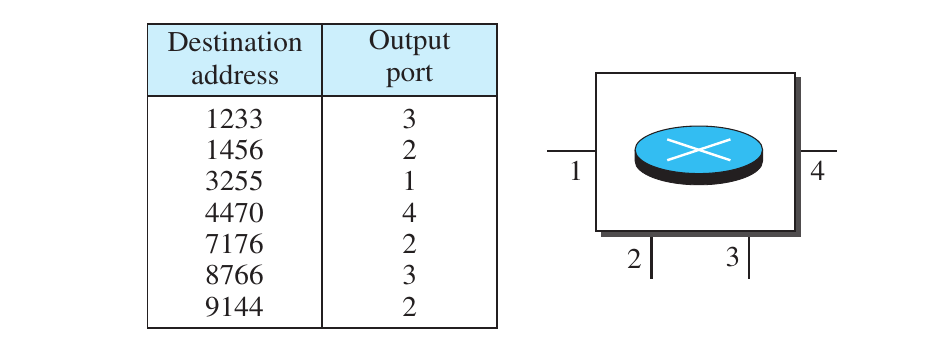
\includegraphics[scale=0.5]{8.27.png}
    \caption{8.27}
\end{figure}
\textbf{Find the output port for packets with the following destination addresses:
\begin{enumerate}
	\item Packet 1: 7176
	\item Packet 2: 1233
	\item Packet 3: 8766
	\item Packet 4: 9144
\end{enumerate}
}

\subsection{Figure 8.28 shows a switch in a virtual-circuit network.}

\begin{figure}[H]
    \center
    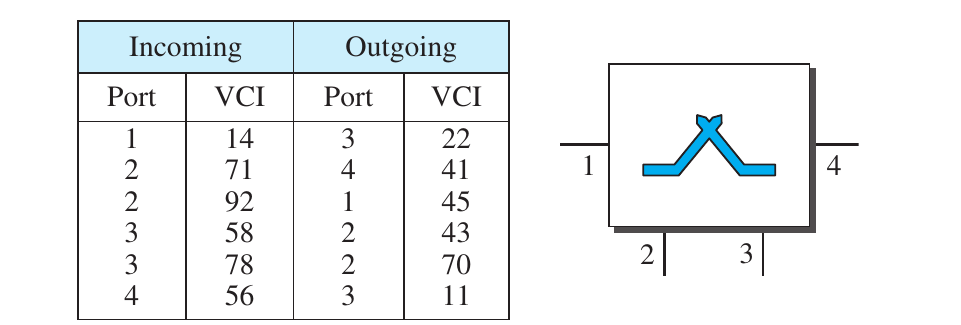
\includegraphics[scale=0.5]{8.28.png}
    \caption{8.27}
\end{figure}
\textbf{Find the output port for packets with the following destination addresses:
\begin{enumerate}
	\item Packet 1: 3, 78
	\item Packet 2: 2, 92
	\item Packet 3: 4, 56
	\item Packet 4: 2, 71
\end{enumerate}
}

\subsection{Answer the following questions:}
\textbf{
	\begin{enumerate}
		\item  Can a routing table in a datagram network have two entries with the same
		destination address? Explain.
		\item Can a switching table in a virtual-circuit network have two entries with the
		same input port number? With the same output port number? With the
		same incoming VCIs? With the same outgoing VCIs? With the same incom-
		ing values (port, VCI)? With the same outgoing values (port, VCI)?
	\end{enumerate}
}

\subsection{It is obvious that a router or a switch needs to search to find information in the
corresponding table. The searching in a routing table for a datagram network
is based on the destination address; the searching in a switching table in a
virtual-circuit network is based on the combination of incoming port and
incoming VCI. Explain the reason and define how these tables must be
ordered (sorted) based on these values.}

\subsection{Consider an n × k crossbar switch with n inputs and k outputs.}

\textbf{
	\begin{enumerate}
		\item  Can we say that the switch acts as a multiplexer if n > k?
		\item Can we say that the switch acts as a demultiplexer if n < k?
	\end{enumerate}
}

\subsection{We need a three-stage space-division switch with N = 100. We use 10 cross-
bars at the first and third stages and 4 crossbars at the middle stage.}

\textbf{
	\begin{enumerate}
		\item  Draw the configuration diagram.
		\item Calculate the total number of crosspoints.
		\item Find the possible number of simultaneous connections.
		\item Find the possible number of simultaneous connections if we use a single
		crossbar (100 × 100).
		\item Find the blocking factor, the ratio of the number of connections in part c
		and in part d.
	\end{enumerate}
}

\subsection{Repeat Problem 8-12 if we use 6 crossbars at the middle stage.}

\subsection{Redesign the configuration of Problem 8-12 using the Clos criteria.}

\subsection{We need to have a space-division switch with 1000 inputs and outputs. What
is the total number of crosspoints in each of the following cases?}
\textbf{
	\begin{enumerate}
		\item  Using a single crossbar.
		\item Using a multi-stage switch based on the Clos criteria.
	\end{enumerate}
}

\subsection{We need a three-stage time-space-time switch with N = 100. We use 10 TSIs
at the first and third stages and 4 crossbars at the middle stage.}
\textbf{
	\begin{enumerate}
		\item  Draw the configuration diagram.
		\item Calculate the total number of crosspoints.
		\item Calculate the total number of memory locations we need for the TSIs.
	\end{enumerate}
}

% \begin{theorem}
%     This is a theorem.
% \end{theorem}

% \begin{proposition}
%     This is a proposition.
% \end{proposition}

% \begin{principle}
%     This is a principle.
% \end{principle}

% Maybe I need to add one more part: Examples.
% Set style and colour later.

% \subsection{Pictures}
% হবে না।
% \begin{figure}[htbp]
%     \center
%     \includegraphics[scale=0.06]{img/photo.jpg}
%     \caption{Sydney, NSW}
% \end{figure}


% \begin{minted}[frame=lines, fontsize=\footnotesize]{python}
%     def hello_world():
%         print("Hello, World!") # This is a comment

%     hello_world()
%     \end{minted}

\end{document}
